\section{Evaluation}

We evaluate \name on a dataset of video streams captured by multiple real-world traffic cameras in a duration of 24 hours. The key findings are the following.
\begin{itemize}
    \item Compared to a baseline of profiling the analytics pipeline just once upfront, \name achieves significantly better performance in both inference accuracy and resource consumption across a variety of accuracy metrics and different times of day (\S\ref{sec:eval:e2e}).
    \item By leveraging the temporal persistence of configurations' inference accuracy, \name can reduce the profiling cost by periodically filtering bad configurations and only checking the top-$k$ best configurations for most of the time  (\S\ref{sec:eval:temporal}).
    \item By leveraging the spatial similarities across video cameras, \name is able to amortize the cost of profiling large configuration spaces across similar cameras with minimal reduction in accuracy (\S\ref{sec:eval:spatial}).
    \item Finally, by assuming the knobs are independent and profiling them separately, \name further cuts the profiling cost
    %by reducing the configuration space to a size linear to the number of choices on each knob  
    (\S\ref{sec:eval:independence}).
\end{itemize}

\subsection{Dataset and setup}

We use a dataset of video streams from five traffic video cameras deployed in different intersections in a metropolitan area. While the cameras share common characteristics (\eg most objects are vehicles moving at a normal speed), the exact content in their video feeds varies significantly over time and across space. 
For instance, day time has more objects and intermittent traffic congestion, while during night time the appearances of objects are more spread out over time. Spatially, as well, two cameras in downtown areas show more cars at slower speeds than other cameras which are deployed in suburbs. In addition, they contain transient car motion patterns when traffic lights change.
Despite their heterogeneity in content, we show \name can opportunistically leverage temporal persistence and spatial similarities between cameras to realize the potential of online configuration adaptation. 
To obtain a representative dataset, we sampled 120 video clips across 24 hours from each camera, and used their original encoded MP4 videos (each being 1280$\times$960p in resolution, 30fps in frame rate, and 150 seconds in length) as the input to test \name. 

The video frames are streamed in their chronological order to the video analytics pipelines, whose configurations are controlled by \name.
The video analytics pipelines expose the control knobs described in \S\ref{sec:pipelines} to \name: 
for Pipeline A: we used 5 levels of frame rate, 4 levels of image size, and 5 pre-trained object detection models; for Pipeline B: we used 5 levels of minimum region size with detected motion, and 5 pre-trained classifier models.
The inference models are implemented in Tensorflow and are pre-trained on standard image datasets~\cite{detectors}, and the switching of video frame rate and resolution is done by FFmpeg~\cite{ffmpeg}.
\jc{add a description on smoothing}

\subsection{End-to-end improvement}
\label{sec:eval:e2e}
We start with the end-to-end improvement of \name over the baseline of one-time update (profiling configurations once at the beginning of a video stream).
Figure~\ref{fig:eval:e2e} shows that for Pipeline A, \name consistently outperforms the baseline along resource consumption and several accuracy metrics for different values of the accuracy threshold $\alpha$. Specifically, we use \emph{bounding box-based} accuracy, where we compute accuracy based on specific locations of objects on the image, and also \emph{label-based} accuracy, where we only compare the \emph{set} of objects on a frame (and ignore locations). Note that the resource (i.e., GPU) consumption includes both profiling of different configuration and running the best configuration to get inference results.

\begin{figure*}[t!]
    \centering
    \hspace{-0.5cm}
    \subfloat[Bounding box-based F1-score over $\alpha=0.8$]
    {
        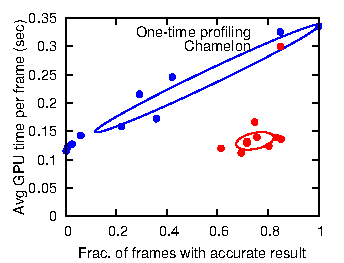
\includegraphics[width=0.33\textwidth]{EvalGraphs/Location_True_Alpha_8.pdf}
        \label{subfig:1}
    }
    \subfloat[Bounding box-based F1-score over $\alpha=0.9$]
    {
        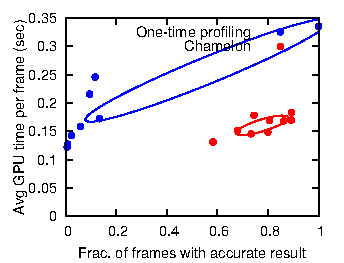
\includegraphics[width=0.33\textwidth]{EvalGraphs/Location_True_Alpha_9.pdf}
        \label{subfig:1}
    }
    \subfloat[Average bounding box-based F1 score]
    {
        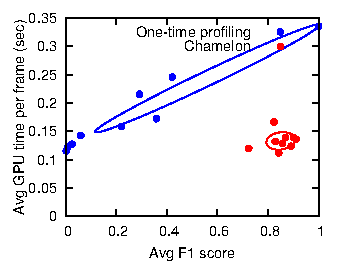
\includegraphics[width=0.33\textwidth]{EvalGraphs/Location_True_Alpha_8_Tradeoff.pdf}
        \label{subfig:1}
    }\\
    \subfloat[Label-based F1-score over $\alpha=0.8$]
    {
        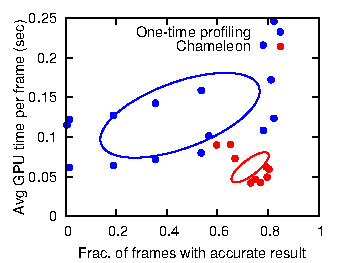
\includegraphics[width=0.33\textwidth]{EvalGraphs/Location_False_Alpha_8.pdf}
        \label{subfig:1}
    }
    \subfloat[Label-based F1-score over $\alpha=0.9$]
    {
        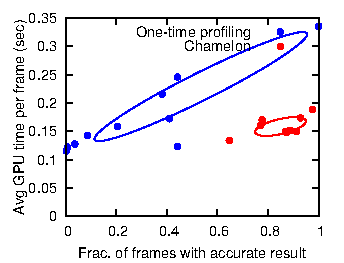
\includegraphics[width=0.33\textwidth]{EvalGraphs/Location_False_Alpha_9.pdf}
        \label{subfig:1}
    }
    \subfloat[Average label-based F1 score]
    {
        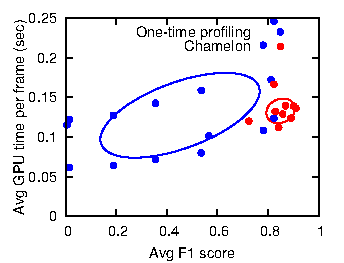
\includegraphics[width=0.33\textwidth]{EvalGraphs/Location_False_Alpha_8_Tradeoff.pdf}
        \label{subfig:1}
    }
    \caption{\name (red) consistently outperforms the baseline of one-time update (blue) across different metrics in Pipeline A. Each dot represents the results of running each solution on one hour of video from five concurrent video feeds. The graphs also include 1-$\sigma$ ellipses to mark the performance variance of each solution.}
    \label{fig:eval:e2e}
    \vskip -8mm
\end{figure*}

We observe improvement on three fronts.
(1) \name achieves 20-50\% higher accuracy while using the same resource consumption, which suggests \name's practical benefit in settings with resource constraints (e.g., edge or mobile devices).
(2) \name achieves 30-50\% reduction in resource consumption (in other words, 2-3x speed up) while achieving almost the same accuracy as the baseline, which could save capital expense when resource are elastic but could be expensive (e.g., cloud VMs).
(3) Finally, \name not only improves the resource consumption and accuracy on average, but also reduces the performance variance: \name's 1-$\sigma$ ellipses are remarkably smaller than those of the baseline\footnote{In many cases, the baseline selected the expensive golden config (top right corner of the graphs), causing the elipses to shift.}. This is because \name is able to continuously adjust its configuration over time while the baseline is sensitive to the starting points of the video. In many scenarios, the baseline would be unusable because it achieves accuracy close to 0.

\begin{figure}[t!]
    \centering
    \hspace{-0.5cm}
    \subfloat[Bounding box-based F1-score over $\alpha=0.8$]
    {
        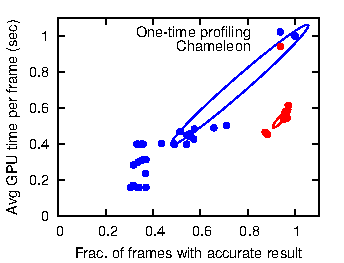
\includegraphics[width=0.24\textwidth]{EvalGraphs_Classifier/Location_True_Alpha_8.pdf}
        \label{subfig:1}
    }
    \subfloat[Label-based F1-score over $\alpha=0.8$]
    {
        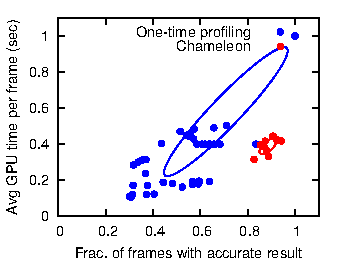
\includegraphics[width=0.24\textwidth]{EvalGraphs_Classifier/Location_False_Alpha_8.pdf}
        \label{subfig:1}
    }
    \caption{\name (red) consistently outperforms the baseline of one-time update (blue) on Pipeline B.}
    \label{fig:eval:e2e-b}
\end{figure}

We also compared \name against the baseline in Pipeline B, and had similar observation. Here, we pick two accuracy metrics and Figure~\ref{fig:eval:e2e-b} shows the comparison between \name and the baseline. Again, \name gives accurate results (F1 score over 0.8) on over 90\% of the frames, while the baseline suffers from higher resource consumption or low accuracy, and a substantial performance variance.



\subsection{Impact of temporal incremental updates}
\label{sec:eval:temporal}
Next, we microbenchmark the impact of individual components in \name. 
We start with the temporal incremental update (\S\ref{subsec:temporal}), and investigate two of its key parameters: the profile window size, and the size of the top-k set.
First, we fix the parameters of \name, and only change the profile window size to see the impact of updating the top-k configurations less often. As observed in \S\ref{subsec:temporal}, the temporal persistence of a configuration's inference accuracy means that reducing the profile frequency (i.e., longer profile windows) should not hurt the performance of the chosen configuration much, at least not for window size less than the typical persistence of a configuration. 
Figure~\ref{subfig:eval:temporal:window} confirms this intuition: 
when we increase the profiling window size from one segment (the top right corner), we see a fast drop in the profiling cost (the gap between the two curves) relative to the degradation in accuracy, until some ``knee point'' (around 3-5 segments) after which any further increase of profiling window size only brings diminishing savings in profiling cost while  reducing accuracy.

Another key factor in temporal incremental update is the size of the top-k best configuration. The intuition is that using a larger top-k set introduces more overhead to check their accuracy in each segment, but tolerates more temporal variance because the best configuration will be more likely to be within the top-k set.
Figure~\ref{subfig:eval:temporal:topk} quantifies this tradeoff as we gradually increase $k$ from 1 (bottom left) to 15 (top right). We observe a good balance in accuracy and resource consumption (mostly dominated by profiling cost), is around $k=5$, below which top-k seems not able to tolerate transient temporal variance (i.e., accuracy degradation), and above which the increased cost of checking top-k set's accuracy does not bring much benefit.

\begin{figure}[t!]
    \centering
    \hspace{-0.5cm}
    \subfloat[Impact of profile window length]
    {
        % 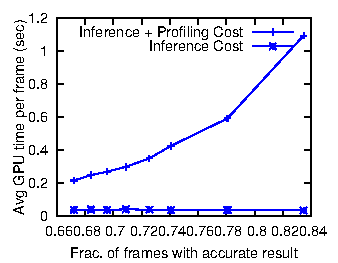
\includegraphics[width=0.24\textwidth]{EvalGraphs/Temporal_Detection_Delta_07.pdf}
        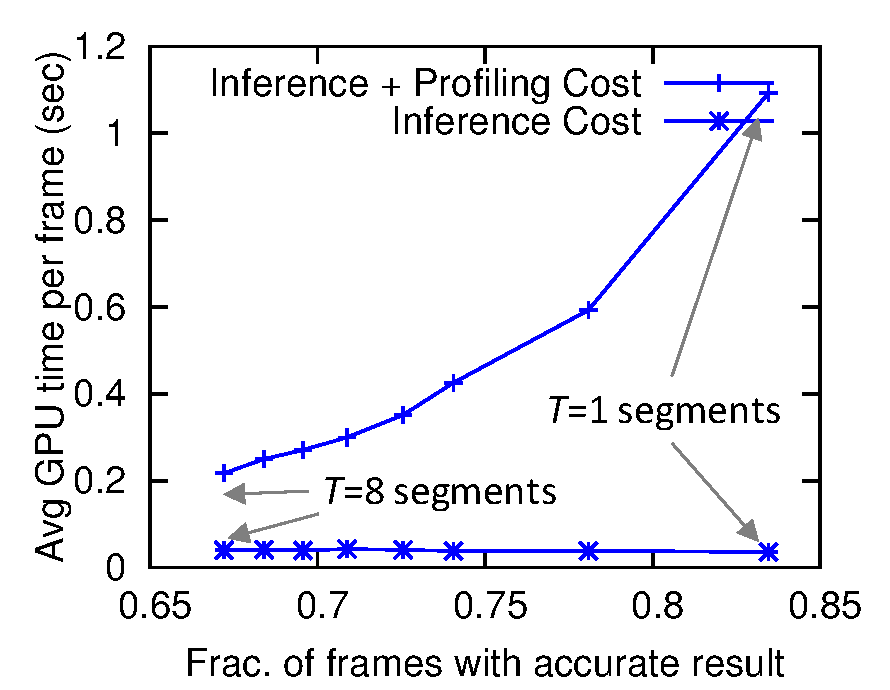
\includegraphics[width=0.24\textwidth]{EvalGraphs/Temporal_new.pdf}
        \label{subfig:eval:temporal:window}
    }
    \subfloat[Impact of top $k$]
    {
        % 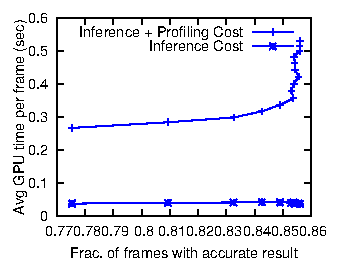
\includegraphics[width=0.24\textwidth]{EvalGraphs/TopK_Detection_Delta_07.pdf}
        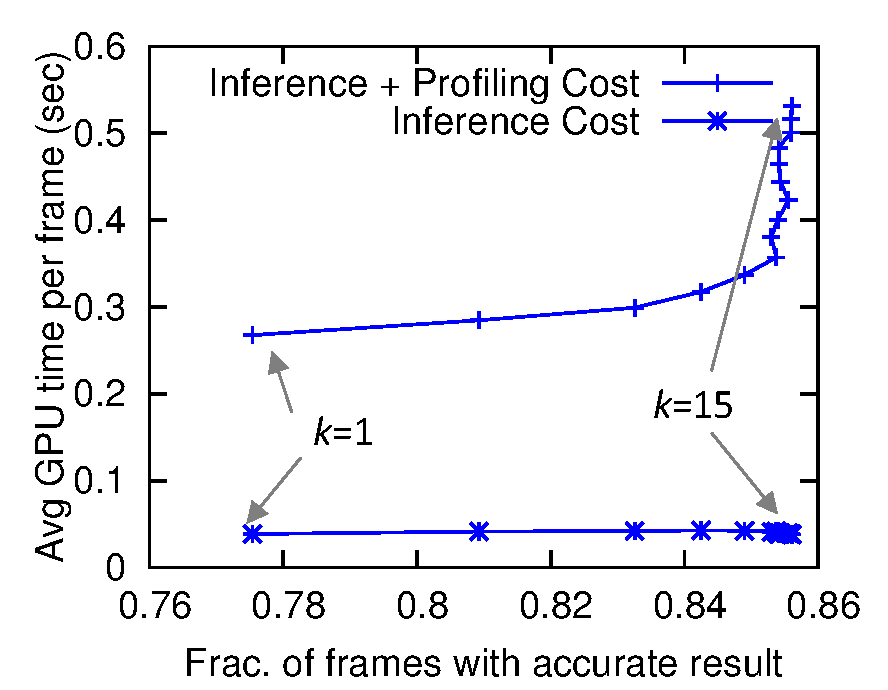
\includegraphics[width=0.24\textwidth]{EvalGraphs/TopK_new.pdf}
        \label{subfig:eval:temporal:topk}
    }
    \caption{Impact of key parameters in temporal incremental update. The accuracy metric is the label-based F1 score with accuracy threshold $\alpha=0.8$.}
    \label{fig:eval:temporal}
\end{figure}


\subsection{Impact of cross-video inference}
\label{sec:eval:spatial}

The second insight behind \name is the existence of multiple cameras sharing characteristics and allowing us to amortize the profiling cost across these similar cameras.
Figure~\ref{fig:eval:spatial} shows the benefits of having more cameras in two cases:
if the cameras are similar, and if the cameras are not all similar. 
Naturally, in the former case, i.e., they share the same set of good configuration at roughly the same time, the cost of profiling should drop almost linearly with the number of cameras. Indeed, Figure~\ref{subfig:eval:spatial:similar} corroborates this intuition. We have ten video feeds\footnote{We created 10 video feeds from 5 cameras by horizontally splitting the view of each camera into two non-overlapping video feeds.} at the same day-time hour, and incrementally add one camera to the test at a time. We observe that \name automatically groups these cameras into one group (using the logic described in \S\ref{subsec:spatial-impl}), and achieves a linear reduction in cost with only small reduction in accuracy.
In contrast, during the hours when the cameras are less similar, we expect to see less reduction of profiling cost, since only a subset of cameras can share the profiling cost. 
This is exactly what happened in Figure~\ref{subfig:eval:spatial:notsimilar}: \name groups the cameras into two (sometimes three) groups, so even though with 10 video feeds, the saving in profiling cost is lower than that in Figure~\ref{subfig:eval:spatial:similar}.

\begin{figure}[t!]
    \centering
    \hspace{-0.5cm}
    \subfloat[More similar cameras]
    {
        % 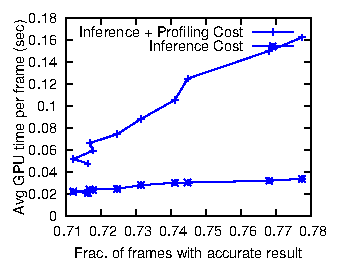
\includegraphics[width=0.24\textwidth]{EvalGraphs/Spatial_Detection_Delta_07.pdf}
        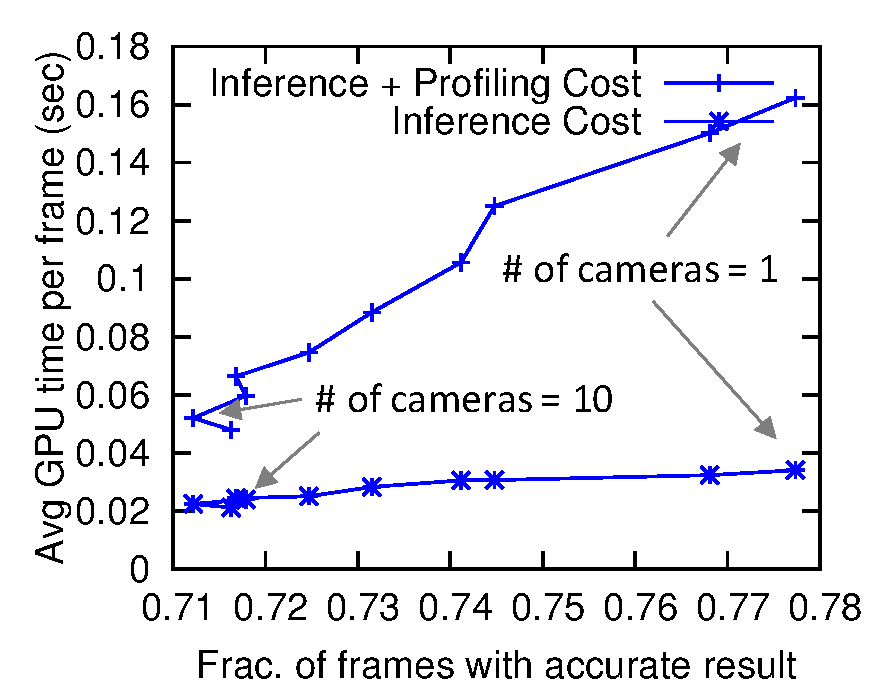
\includegraphics[width=0.24\textwidth]{EvalGraphs/Spatial_new1.pdf}
        \label{subfig:eval:spatial:similar}
    }
    \subfloat[More cameras that are not all similar]
    {
        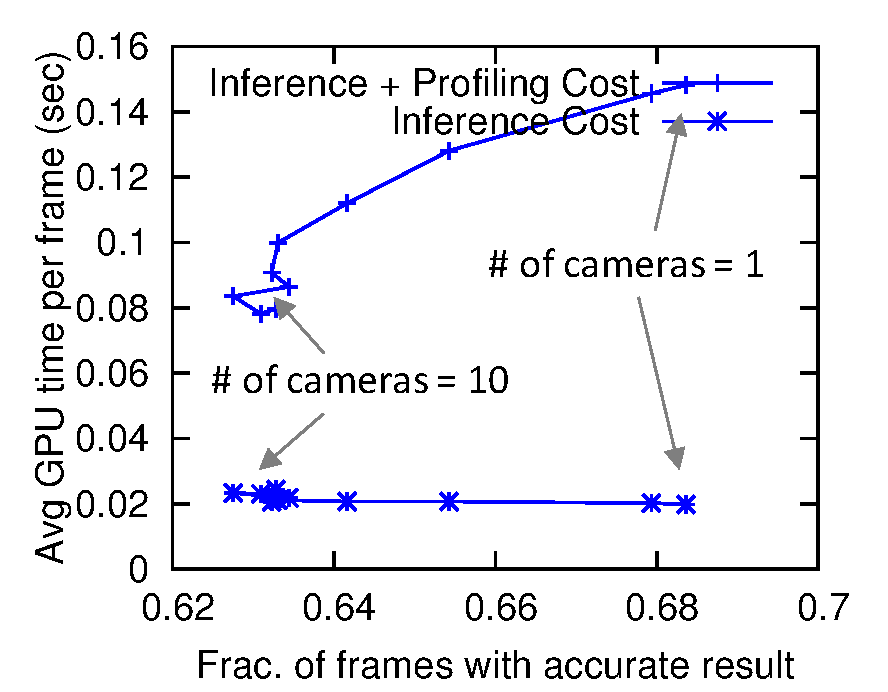
\includegraphics[width=0.24\textwidth]{EvalGraphs/Spatial_new2.pdf}
        \label{subfig:eval:spatial:notsimilar}
    }
    \caption{The benefit of having more cameras.}
    \label{fig:eval:spatial}
    \vspace{-3pt}
\end{figure}


\subsection{Impact of reducing configuration spaces}
\label{sec:eval:independence}

The last key technique in \name is to reduce the cost of profiling the configuration space once by profiling the knobs separately.
The reduction in profiling cost is obvious, but the impact on accuracy and inference cost of the picked configuration is less evident. 
In Figure~\ref{fig:eval:independence}, we compare the configurations found by Algorithm~\ref{alg:policy3} (based on the assumption that knobs are independent) and the exhaustive search (which is supposed to find better configurations if the knobs are not completely independent) along three metrics:
accuracy (Figure~\ref{subfig:eval:independence:accuracy}), inference cost  (Figure~\ref{subfig:eval:independence:pickedcost}) of the configurations picked by each algorithm, and the profiling cost required to execute the  algorithms
(Figure~\ref{subfig:eval:independence:profilingcost}).
We can see that the configurations picked by Algorithm~\ref{alg:policy3} is almost as good as the result of running an exhaustive search (in terms of accuracy and inference cost), and at the same time, it achieves an enormous reduction in the profiling cost.


\begin{figure}[t!]
    \centering
    \hspace{-0.5cm}
    \subfloat[Accuracy]
    {
        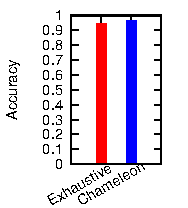
\includegraphics[width=0.17\textwidth]{EvalGraphs/Independence_Detection_Accuracy.pdf}
        \label{subfig:eval:independence:accuracy}
    }
    \subfloat[Inference cost]
    {
        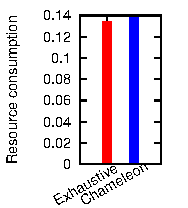
\includegraphics[width=0.17\textwidth]{EvalGraphs/Independence_Detection_PickedCost.pdf}
        \label{subfig:eval:independence:pickedcost}
    }
    \subfloat[Profiling cost]
    {
        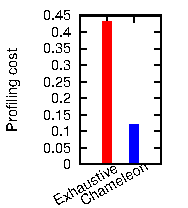
\includegraphics[width=0.17\textwidth]{EvalGraphs/Independence_Detection_ProfilingCost.pdf}
        \label{subfig:eval:independence:profilingcost}
    }
    \caption{Comparing the profiling algorithm of Chameleon (Algorithm~\ref{alg:policy3}) with the result of the exhaustive search.}
    \label{fig:eval:independence}
\end{figure}

\subsection{Contribution of each component}

Finally, we investigate the incremental contribution of individual techniques in \name, by incrementally adding one technique at a time (temporal incremental update, spatial cross-camera inference, and using knob independence).
Figure~\ref{fig:eval:contrib} shows the performance of full \name as well as that of some intermediate design points in the two pipelines under our consideration.
First, we see that each step brings significant reduction in cost at a relatively small drop in accuracy.
Incremental update reduces profiling cost by about $\sim$50\%, cross-camera inference by additional $\sim$30-60\%, and finally, the independence assumption by another 40-60\%.
Second, we note that the reduction in resource consumption in Pipeline A is a smaller cost in accuracy (though with a slightly higher variance) than in Pipeline B. 
The reason is in general the tradeoff between accuracy and resource consumption is more favorable in Pipeline A than in Pipeline B; in other words, using cheaper configuration in A does not necessarily has a large cost in accuracy, so it has more the room to reduce cost at a minimal price in accuracy.

\begin{figure}[t!]
    \centering
    \hspace{-0.5cm}
    \subfloat[Pipeline A]
    {
        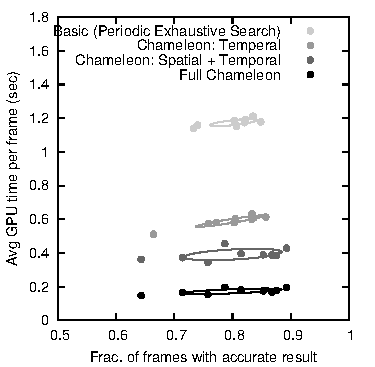
\includegraphics[width=0.24\textwidth]{EvalGraphs/PuttingTogether.pdf}
        \label{subfig:eval:contrib:A}
    }
    \subfloat[Pipeline B]
    {
        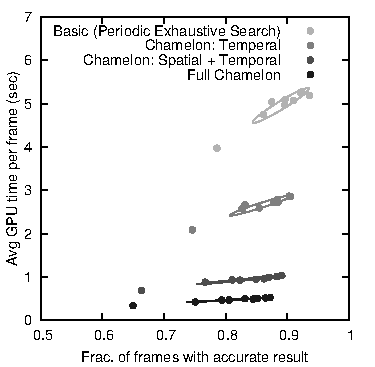
\includegraphics[width=0.24\textwidth]{EvalGraphs_Classifier/PuttingTogether.pdf}
        \label{subfig:eval:contrib:B}
    }
    \caption{Contribution of individual components}
    \label{fig:eval:contrib}
\end{figure}